\documentclass[tikz,border=10pt]{standalone}
\usetikzlibrary{positioning}

\usepackage{tikz}
\usetikzlibrary{arrows.meta, decorations.markings}

\tikzset{
    midarrow/.style={
        decoration={markings, mark=at position 0.53 with {\arrow{Latex}}},
        postaction={decorate}
    }
}

\begin{document}
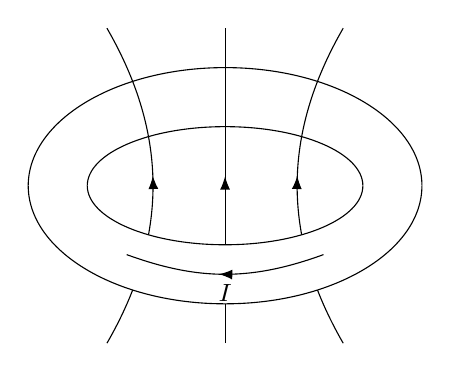
\begin{tikzpicture}
	\def\Rx{2.5}
	\def\rx{1.75}
	\def\Ry{1.5}
	\def\ry{0.75}

	\draw (-\rx,0) [x radius=\rx cm, y radius=\ry cm]
	arc[start angle=180, end angle=0];
	\draw (\Rx,0) [x radius=\Rx cm, y radius=\Ry cm]
	arc[start angle=0, end angle=180];

	\def\anglediff{30}
	\def\sepx{1.5}
	\draw[midarrow]
	(-\sepx, -2)
	to [out=90-\anglediff, in=-90+\anglediff]
	(-\sepx,2);
	\draw[midarrow]
	(0, -2)
	to [out=90, in=-90]
	(0,2);
	\draw[midarrow]
	(\sepx, -2)
	to [out=90+\anglediff, in=-90-\anglediff]
	(\sepx,2);

	\fill[white] (-\rx,0) [x radius=\rx cm, y radius=\ry cm]
	arc[start angle=180, end angle=360] --
	(\Rx,0) [x radius=\Rx cm, y radius=\Ry cm]
	arc[start angle=360, end angle=180] -- cycle;

	\draw (-\rx,0) [x radius=\rx cm, y radius=\ry cm]
	arc[start angle=180, end angle=360];
	\draw (\Rx,0) [x radius=\Rx cm, y radius=\Ry cm]
	arc[start angle=360, end angle=180];

	\draw[midarrow]
	(\Rx/2, -\Ry/3-\ry/2)
	to [out=200, in=-20]
	(-\Rx/2, -\Ry/3-\ry/2);
	\node[anchor=north] at (0, -\Ry/2-\ry/2) {\small \( I \)};
\end{tikzpicture}

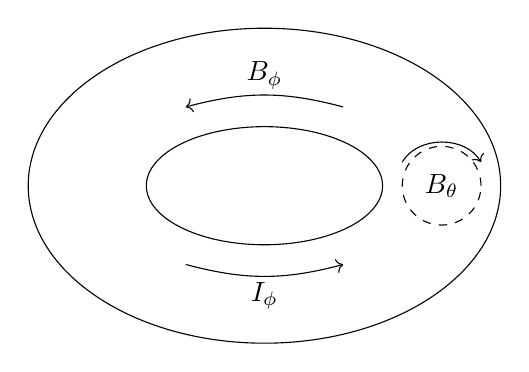
\begin{tikzpicture}
	\draw (0,0) ellipse [x radius=3cm, y radius=2cm];
	\draw (0,0) ellipse [x radius=1.5cm, y radius=0.75cm];
	\draw[dashed] (2.25,0) circle [radius=0.5cm];

	\draw[->]
	(1.75,0.3)
	to [out=60, in=120]
	(2.75,0.3);

	\node at (2.25, 0) {\( B_\theta \)};

	\draw[->]
	(1,1)
	to [out=165, in=15]
	(-1,1);

	\node at (0, 1.4) {\( B_\phi \)};

	\draw[->]
	(-1,-1)
	to [out=-15, in=195]
	(1,-1);

	\node at (0, -1.4) {\( I_\phi \)};
\end{tikzpicture}
\end{document}
